%to have line numbers
%\RequirePackage{lineno}
\documentclass[10pt, letterpaper]{article}      
\usepackage[margin=.1cm,font=small,labelfont=bf]{caption}[2007/03/09]
%\usepackage{endnotes}
%\let\footnote=\endnote


\usepackage{setspace}
\usepackage{longtable}                        
\usepackage{anysize}                          
\usepackage{natbib}                           
%\bibpunct{(}{)}{,}{a}{,}{,}                   
\bibpunct{(}{)}{,}{a}{}{,}                   
\usepackage{amsmath}
\usepackage[% draft,
pdftex]{graphicx} %draft is a way to exclude figures                
%\usepackage{epstopdf}
\usepackage{hyperref}                             % For creating hyperlinks in cross references
 
% \usepackage[margins]{trackchanges}

% \note[editor]{The note}
% \annote[editor]{Text to annotate}{The note}
%    \add[editor]{Text to add}
% \remove[editor]{Text to remove}
% \change[editor]{Text to remove}{Text to add}

%TODO make it more standard before submission: \marginsize{2cm}{2cm}{1cm}{1cm}
\marginsize{1cm}{1cm}{.5cm}{.5cm}%{left}{right}{top}{bottom}   
					          % Helps LaTeX put figures where YOU want
 \renewcommand{\topfraction}{1}	                  % 90% of page top can be a float
 \renewcommand{\bottomfraction}{1}	          % 90% of page bottom can be a float
 \renewcommand{\textfraction}{0.0}	          % only 10% of page must to be text

 \usepackage{float}                               %latex will not complain to include float after float

\usepackage[table]{xcolor}                        %for table shading
\definecolor{gray90}{gray}{0.90}
\definecolor{orange}{RGB}{255,128,0}

\renewcommand\arraystretch{.9}                    %for spacing of arrays like tabular

%-------------------- my commands -----------------------------------------
\newenvironment{ig}[1]{
\begin{center}
 %\includegraphics[height=5.0in]{#1} 
 \includegraphics[height=3.3in]{#1} 
\end{center}}

 \newcommand{\cc}[1]{
\hspace{-.13in}$\bullet$\marginpar{\begin{spacing}{.6}\begin{footnotesize}\color{blue}{#1}\end{footnotesize}\end{spacing}}
\hspace{-.13in} }

%-------------------- END my commands -----------------------------------------



%-------------------- extra options -----------------------------------------

\usepackage{pdfpages} %load after xcolor, like at the end ideally i guess and
                      %turn off epstopdf


%%%%%%%%%%%%%
% footnotes %
%%%%%%%%%%%%%

%\long\def\symbolfootnote[#1]#2{\begingroup% %these can be used to make footnote  nonnumeric asterick, dagger etc
%\def\thefootnote{\fnsymbol{footnote}}\footnote[#1]{#2}\endgroup}	%see: http://help-csli.stanford.edu/tex/latex-footnotes.shtml

%%%%%%%%%%%
% spacing %
%%%%%%%%%%%

% \abovecaptionskip: space above caption
% \belowcaptionskip: space below caption
%\oddsidemargin 0cm
%\evensidemargin 0cm

%%%%%%%%%
% style %
%%%%%%%%%

%\pagestyle{myheadings}         % Option to put page headers
                               % Needed \documentclass[a4paper,twoside]{article}
%\markboth{{\small\it Politics and Life Satisfaction }}
%{{\small\it Adam Okulicz-Kozaryn} }

%\headsep 1.5cm
% \pagestyle{empty}			% no page numbers
% \parindent  15.mm			% indent paragraph by this much
% \parskip     2.mm			% space between paragraphs
% \mathindent 20.mm			% indent math equations by this much

%%%%%%%%%%%%%%%%%%
% extra packages %
%%%%%%%%%%%%%%%%%%

\usepackage{datetime}


\usepackage[latin1]{inputenc}
\usepackage{tikz}
\usetikzlibrary{shapes,arrows,backgrounds}


%\usepackage{color}					% For creating coloured text and background
%\usepackage{float}
\usepackage{subfig}                                     % for combined figures

\renewcommand{\ss}[1]{{\colorbox{blue}{\bf \color{white}{#1}}}}
\newcommand{\ee}[1]{\endnote{\vspace{-.10in}\begin{spacing}{1.0}{\normalsize #1}\end{spacing}\vspace{.20in}}}
\newcommand{\emd}[1]{\ExecuteMetaData[/tmp/tex]{#1}} % grab numbers  from stata

%TODO before submitting comment this out to get 'regular fornt'
\usepackage{sectsty}
\allsectionsfont{\normalfont\sffamily}
\usepackage{sectsty}
\allsectionsfont{\normalfont\sffamily}
\renewcommand\familydefault{\sfdefault}

% \usepackage[margins]{trackchanges} (LM)
\usepackage{rotating}
\usepackage{catchfilebetweentags}

\usepackage{abstract}
\renewcommand{\abstractname}{}    % clear the title
\renewcommand{\absnamepos}{empty} % originally center
%-------------------- END extra options -----------------------------------------
\date{{}\today}
\title{  % remember to have Vistula University!!
Elderly Volunteering and Well-Being in Europe. Revisting Haski (2009) \footnote{This study was funded by grant \# 2016/21/B/HS4/03058 from
  Polish National Science Foundation (Narodowe Centrum Nauki).}
}
\author{
Adam Okulicz-Kozaryn\thanks{EMAIL: adam.okulicz.kozaryn@gmail.com
  \hfill I thank XXX.  All mistakes are mine.} \\
{\small Rutgers - Camden  and Vistula University}
}

\begin{document}

%%\setpagewiselinenumbers
%\modulolinenumbers[1]
%\linenumbers

\bibliographystyle{/home/aok/papers/root/tex/ecta}
\maketitle
\vspace{-.4in}
\begin{center}

\end{center}


\begin{abstract}
\noindent
\end{abstract}
\vspace{.15in} 
\noindent{\sc XXX TODO add to ebib as keyword PAPER-CODE-NAME and tag with ebib keywords 
}
\vspace{.25in} 

\begin{spacing}{1.4} %TODO MAYBE before submission can make it like 2.0
\rowcolors{1}{white}{gray90}

%  instead \ExecuteMetaData[../out/tex]{ginipov} do \emd{ginipov}

% \begin{figure}[H]
%  \includegraphics[height=3in]{../out/gov_res_trust.pdf}\centering\label{gov_res_trust}
% \caption{woo}
% \end{figure}


%TODO !!!! have input here aok_var_des
%%%%%%%%%%%%%%%%%%%%%%%%%%%%%%%%%%%%%%%%%%%%%%%%%%%%%%%%%%%%%%%%%%%%%%%%%%%%%%

Haski (2009) is a rare example of a data driven study on volunteerism among elderly. She used data from the first wave of Survey of Health, Ageing and Retirement in Europe (SHARE) to analyze volunteering among people aged 50 in 12 Western and Southern European countries.  The paper includes an extensive discussion of variations in volunteering rates according to main socio-economic variables as age, gender and employment status in included countries and it finds positive relation between volunteering and physical and psychological well-being. She concluded that volunteering rates differed according to country  in the way known from earlier studies with the highest rates in Northern Europe and the lowest rates in Southern Europe . The same result can be found in Erlinghagen and Hank  (2006).  Haski (2009) identified  positive correlation of  volunteerism  with perceived health, life satisfaction, and self-life expectancy and a negative correlation to depression.  However, the most puzziling part of the paper is on no clear relation between impact of volunteering on health and quality of life and extend of volunteering. For example, it is reported that the Pearson correlation  between volunteering and health in Italy  is 0.114, while in the Netherlands it is lower 0.090. \\

The paper extends the study by Haski (2009) in a few directions. In the mentioned paper the first wave of Survey of Health, Ageing and Retirement in Europe (SHARE) was used. Those data were collected in 2004 and 2005. Our study uses data collected in 2015 in the sixth wave of the SHARE survey. Thanks to that we may add some  Central and Eastern European countries (CEE) into the analysis that were not previously  analyzed they were not included in the first wave of the survey. This  leads to new insights since life course of population of 50+ in CEE is remarkable different to the experience of people from Western Europe. This is important since despite that the study is a line of research focusing on cross-country comparisons it adds countries that have not been analysed so far. Secondly, in the first wave of the SHARE survey volunteering was identified through a question on activities conducted during last 4 weeks before the interview. Starting from the wave 4 the question asks about activities in 12 months preceding the interview. This was important change making the volunteering rates calculted from the SHARE data more similar to the statistics from other sources.  Third, association between volunteering and health or life satisfaction is measured in the paper by the Kendall tau coefficient while Haski (2009) used the Pearson correlations. Also, we test statistical significance of differences in the correlations between countries while the previous discussion was solely based on informal discussion.  Taking into account that differences in the correlation coefficients are often small it is not obvious if a given difference is really meaningfull. Finally, we use different measures of life satisfaction (quality of life) and health to ones used in the reference paper.  \\

In the paper we concentrate on the relation between the extend of volunteerism and its impact on life satisfaction. We hypotesis that such relation can be nonlinear with lower values in countries with low or high volunnteering rates and higher rates in countries with mid range of volunteerism. A second topic disccused below is a relation between an impact from volunteering on subjective health and a popularity of volunteerism. \\


Finally, our results have interesting practical values. Population aging in Europe is a fact, and it asks for new policy tools that may be used to keep elderly wellbeing on decent levels. We suggest that volunteerism is an interesting option in that regard but there are limits to the way how volunteering can increase life satisfaction.  
 
\section{Literature}

A list of empirical papers on volunteerism among elderly (Erlinghagen and Hank, 2006; Wahlendorf and Siegriest, ?) //

CO TUTAJ UWZGLEDNIC ? //

Volunteering differently influences life satisfaction over life course. Willigen (2000) notices that "...elderly experience greater positive changes in their perceived health than did younger adult volunteer". Volunteering changes with age not only in its popularity but also in its characteristics (Lit. ). The motives are also presumably different.  One may to take a  macroeconomic perspective and to distinguish between demand side and supply side explanations (Ziemek, 2006). 

Country differences in volunteering rates //
Demand for volunteering may be created by unmet demand for public goods and services that are not delivered by either the market or the government (Weisbroad, 1997). The supply side explanation stress a role of a person who allocates her or his time to unpaid activities to improve on either a current supply or to create it. Both perspectives  suggests that volunteering should be related to rather unsatisfactory level of supply of public good and services. This suggests that it should be more popular in less developed countries. However, this prediction is false and volunteering is rather positively  related to the degree of economic development (Haski, 2009, ...) what is suggesting a considerable role of supply factors in explaining the differences in the rates of volunteering among elderly. The significance of supply side factors stress the role of traditional economic determinants as health and income but it does not eliminate preferences or culture from the analysis. Despite factors explaining demand for and supply of hours devoted to volunteering  we need to remeber about a matching mechanizm that needs to exist if we want to observe volunteering. By the assumption a market mechanizm based on a price signal is not a good candidate for it. It is natural to expect that quality of goverment will have an important role in explaining country differences in popularity of volunteering. The role of state policy is important for overcoming the barriers to volunteering realted to transport difficulties, lack of information, perceptions of volunteering and lack of variety in the opportunities \footnote{Older People Volunteering: Literature Review, 2009, Northern Irleand}. The matching requirement may help to understand why volunteerism is more popular in better developed countries.  This relation between economic development and rates of volunteering is true for elderly, also.  This is seen for example in OECD data.\\

\begin{figure}[H]
 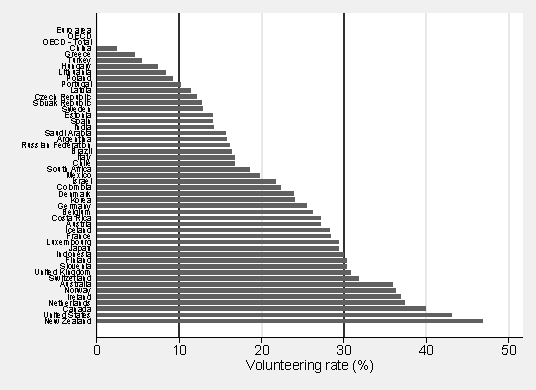
\includegraphics[height=3in]{oecd_age50p.pdf}
 \centering
 \label{fig:oecd_50p}
\caption{volunteering shares}
\end{figure}

Health \\
The literature describing relation (or correlation) between engagement in volunteering and subjective health or life satisfaction is quite rich (LIT). For example Jenkins et al. (2013) surveyed forty experimental and cohort studies comparing the physical and mental health outcomes and mortality of a volunteering group to a non-volunteering group. They concluded that volunteering had favourable effects on depression, life satisfaction, wellbeing but not on physical health. Also, factors such as altruism and reciprocity were presented as core components explaining motivation for engaging in unpaid activities. \\

Wellbeing, life satisfaction, \\

1. Borgonovi(2008) - showed that voluntary work is associated with better self-assessed health and higher levels of happiness \\
2. Meier and Stutzer (2008) showed that volunteering led to increased life satisfaction in a longitudinal study in Germany. \\
3. Casiday et al (2008) noted that the majority of the papers their review covered were based on data from the United States, and they identified the need for further research in the UK. \\
4. James Nazroo and Katey Matthews (2012): As hypothesised, the improvement in well-being is only present for those who feel rewarded for the efforts they put into volunteering (Table 3), page 27. \footnote{ The impact of volunteering on well-being in later life, A report to WRVS}

\textit{Here: main conclusion from this literature}. Much less is known about how important is engagement in volunteering  for well-being. 

Duzo info w sieci haslo "volunteerism among elderly" \\
http://longevity.stanford.edu/2016/11/03/engaging-in-volunteerism-may-hold-significant-health-benefits/

\section{Data}

\textbf{About SHARE} \\
We use from the 2015 Survey of Health, Ageing and Retirement in Europe (SHARE). The dataset provides wide range of information on the socio-economic status, health, and family relationships of people in age 50 or more in XY European countries. The wave 6 used in the research is based on XXXXX interviews (CAPI) in 12 countries that were included in the wave 1 (Austria, Belgium, Denmark, France, Germany, Greece, Israel, Italy, Spain, Sweden, Switzerland, and The Netherlands) and 9 countries that entered the survey later on (Czech Republic, Poland, Ireland, Luxembur, Hungary, Portugal, Slovenija, Estonia and Croatia). Over 68 000 elderly  participated in the survey. SHARE applies a concept of ex-ante harmonisation: there is one common generic questionnaire that is translated into the national languages using an internet based translation tool and processed automatically in a common CAPI instrument. \\

Sampling \\
Probability samples were drawn in each participating country. Due to different institutional conditions a uniform sampling design was impossible. For example, a simple random selection of
households, from the central population register was used in in Denmark, while complex multistage design was applied in Greece. The weighted average household response rate was
XX\%, and ranged from XX\% in CC to 74\% in CC. 


\textbf{volunteering //}
Volunteering is identified solely on a basis of respondent's declaration about activities conducting in last 12 months. The question was phrased: "Have you done any of these activities in the last month: Done voluntary or charity work." The variable was recoded into a binary variable with the value one for those indicating that activity. Volunteering considered in the study does not include a help given to close family members. This understanding of the volunteering is consistent with the UN definition \footnote{United Nations Volunteers Programme: Preparatory Committee for the Special Session of the General Assembly on the implementation of the outcome of the world summit for social development and further initiatives. Volunteering and social development. A/AC.253/16/Add.7. United Nations; 2000.}. However, one needs to remember that our volunteering measure is not free of possibility of being condaminated by a measurement error. 

Another widely accepted feature of formal volunteerism is that, it takes place within a formal organisational structure, is self-governing, is not profit distributing (?) and is independent of government (Salamon and Sokolowski 2001). Another way of defining voluteering is "informal" volunteering conducted outside of the structures of a voluntary organisation such as providing unpaid help to a friend or neighbour. Informal volunteering includes activities that are very heterogeneous. We are aware that informal and formal volunteering may have very different impact on individuals well being. In the study we include only formal volunteering. Informal is identified in separate question (check to be sure)

\textbf{Quality of life, life satisfaction, CASP} \\
Our measure of life satisfaction differs from the one applied in Haski(2009). We use the CASP-12 index described in details in (Hyde, M. (2003) A measure of quality of life in early old age: The theory, development and properties of a needs satisfaction model (CASP-19). Aging and mental health, 7 (3), 186-194.).


\textbf{health} \\
We use similar measure of subjective health to the one used in Haski(2009). This is the self-perceived health variable with the respondents that range from "very bad" to "very good". 


\section{Results}

\subsection{Result 1: volunteering rates}

The way how question on volunteering was formulated in the SHARE had significant impact on levels of the rates. The graph below compares the rates from Haski (2009) and the rates calculated using the wave 6 with the rates reported in OECD(2016). [to nie jest dobra prezentacja, ale informacja jest potrzebna]

\begin{figure}[H]
 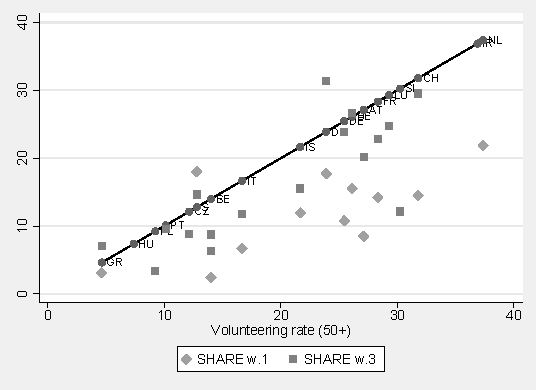
\includegraphics[height=3in]{oecd_oecdShare16.pdf}
 \centering
 \label{fig:volshares}
\caption{volunteering shares}
\end{figure}

For all countries included in the wave 1 and in the wave 6 the rates from the later study are closer to those published by the OECD. Also, the rates from the wave 6 exceeds that those from the wave 1 except Sweden (18\% vs. 15\%).  For example, for Switzerland the rate has increased from less than 15\% up to almost 30\%. In Germany the change has been from 17\% to almost 25\%. The rates for countries that did not particpated in the wave 1 are low - Poland 3.43\%, Czech Republic 8.87\%, Estonia 8.75\%, Portugal 9.55\%, Slovenia 12.15\%. Only for Luxemburg the rate is high - 24.75\%. \\

Similar to previous studies, the analysis showed that volunteering rates varied according to country. The pattern is as usuall - the highest rates 
were found in Northern and Western Europe:  Denmark (31.4\%), Switzerland (29.5\%) and Belgium (26.6\%). The lowest rates of volunteering were found in Eastern and Southern Europe: Poland (3.4\%), Spain (6.3\%), Greece (7.0\%) and Czech Republic (8.9\%). \\

Changes in the question made volunteering rates in the SHARE more similar to those published by the OECD using the Gallup data. Two additional "things" should be observed. First, even though levels in the OECD and in the SHARE data are different the divison into low valued Southern and Central Europe and high valued Western and Northern Europe is consistent. Second, results for Sweden \textit{are somehow couterintuitive. Lower values in the wave 6 than in the wave 1 suggest that less elderly were egaged in volunteering in 2015 than in 2006. ??? }


\subsection{Result 2: Kendall-tau and significance test - volunteering vs. subjective health and casp}

The Kendall tau is a measure of association between two ordinal variables. When observations have similar ranks the value of the measure rises, and have they have dissimilar ranks it is low. \textbf{czy tyle starczy ? czy bardziej opisywac metode ?} \\

Values for the Kendall tau(b) correlations are given in the appendix. Below pvalues for pair wise comparisons are presented.\footnote{First row: the volunteering rate, second row: taub correlation; change ordering in the health variable } 

%%% TABLE
\begin{spacing}{.9}
	 % Table generated by Excel2LaTeX from sheet 'Health'
\begin{table}[H]
  \centering
  \caption{Volunteering and health (taub): pvalues}
    \begin{tabular}{lrrrrrrrrrrrrr}
          & \multicolumn{1}{c}{AT} & \multicolumn{1}{c}{FR} & \multicolumn{1}{c}{BE} & \multicolumn{1}{c}{CH} & \multicolumn{1}{c}{DE} & \multicolumn{1}{c}{DK} & \multicolumn{1}{c}{CZ} & \multicolumn{1}{c}{IT} & \multicolumn{1}{c}{SE} & \multicolumn{1}{c}{PL} & \multicolumn{1}{c}{IS} & \multicolumn{1}{c}{GR} & \multicolumn{1}{c}{S} \\
          & \multicolumn{1}{c}{0.201} & \multicolumn{1}{c}{0.229} & \multicolumn{1}{c}{0.266} & \multicolumn{1}{c}{0.295} & \multicolumn{1}{c}{0.239} & \multicolumn{1}{c}{0.314} & \multicolumn{1}{c}{0.089} & \multicolumn{1}{c}{0.118} & \multicolumn{1}{c}{0.147} & \multicolumn{1}{c}{0.034} & \multicolumn{1}{c}{0.155} & \multicolumn{1}{c}{0.07} & \multicolumn{1}{c}{0.063} \\
          & \multicolumn{1}{c}{-0.162} & \multicolumn{1}{c}{-0.125} & \multicolumn{1}{c}{-0.123} & \multicolumn{1}{c}{-0.121} & \multicolumn{1}{c}{-0.112} & \multicolumn{1}{c}{-0.099} & \multicolumn{1}{c}{-0.085} & \multicolumn{1}{c}{-0.082} & \multicolumn{1}{c}{-0.081} & \multicolumn{1}{c}{-0.073} & \multicolumn{1}{c}{-0.04} & \multicolumn{1}{c}{-0.021} & \multicolumn{1}{c}{-0.017} \\
    AT    &       &       &       &       &       &       &       &       &       &       &       &       &  \\
    FR    & 0.079 &       &       &       &       &       &       &       &       &       &       &       &  \\
    BE    & 0.045 & 0.904 &       &       &       &       &       &       &       &       &       &       &  \\
    CH    & 0.071 & 0.845 & 0.92  &       &       &       &       &       &       &       &       &       &  \\
    DE    & 0.015 & 0.497 & 0.539 & 0.675 &       &       &       &       &       &       &       &       &  \\
    DK    & 0.003 & 0.202 & 0.208 & 0.33  & 0.528 &       &       &       &       &       &       &       &  \\
    CZ    & 0     & 0.041 & 0.036 & 0.098 & 0.168 & 0.49  &       &       &       &       &       &       &  \\
    IT    & 0     & 0.022 & 0.017 & 0.064 & 0.108 & 0.38  & 0.864 &       &       &       &       &       &  \\
    SE    & 0     & 0.017 & 0.013 & 0.053 & 0.09  & 0.341 & 0.811 & 0.946 &       &       &       &       &  \\
    PL    & 0     & 0.029 & 0.027 & 0.061 & 0.101 & 0.283 & 0.601 & 0.688 & 0.723 &       &       &       &  \\
    IS    & 0     & 0.001 & 0.001 & 0.003 & 0.005 & 0.025 & 0.076 & 0.091 & 0.098 & 0.258 &       &       &  \\
    GR    & 0     & 0     & 0     & 0     & 0     & 0     & 0.001 & 0.001 & 0.001 & 0.027 & 0.446 &       &  \\
    S     & 0     & 0     & 0     & 0     & 0     & 0     & 0.001 & 0.001 & 0.001 & 0.022 & 0.383 & 0.864 &  \\
    \end{tabular}%
  \label{tab:addlabel}%
\end{table}%

      \label{tauH} 
\end{spacing}
%%%% END: TABLE

In all countries volunteering is associated with better subjective health. The highest correlation is for Austria (16.2\%)and it is statistically different to any other coefficient. The correlations in France, Belgium, Switzerland, Germany and Denmark range from 12.5\% to 9.9\% and all pairs are statistically indifferent. Another group in which all pairs are statistically indifferent consists on Denmark, Czech Republic, Italy, Spain and Poland. The correlation range here from 9.9\% to 3.4\% (Poland). The coefficients are not significantly different also between Poland and Isreal and Isreal, Greece and Sweden.\footnote{Isreal - if we remove it we will get more clarity} 

The ordering is not complete but it leads to some intresting suggestions. As we see the association between volunteering and health is stronger in Western Europe where the rates are high than in Southern and East Europe. One may for example state that the associations in Poland and in Czech Republic are lower than  in any Western European country except Sweden. The same relation occures between Western European countries and Southern European countries. Also, it is intresting to note that results for Austria and Sweden are unexpected. In the first case the correlation is too strong what makes it different from economically similar countries, while in Sweden the coefficient is lower than one would exepct it to be.  \\

Putting aside outliers like Austria and Sweden associations between volunteering and health as measured by the differences in Kendall tau b coefficient seem to reflect quite closely the differences in economic development.  One may view the above results as a suggestion that Europe is divided into three parts: highly developed Europe (AT, FR, BE, CH, DE), countries in the middle  (DK, CZ, IT), and countries behind (ES, PL, GR).  \\

The bottom line here is that volunteering and subjective health are related differently in different countries and that these differences are realted to the economic development and to the popularity of volunteering in a country. [?]

The pvalues for the significance tests of the Kendall correlations between volunteering and life satisfaction are given in table X.  \\


%%% TABLE
\begin{spacing}{.9}
	 % Table generated by Excel2LaTeX from sheet 'Lilfe Sat.'
\begin{table}[H]
  \centering
  \caption{Add caption}
    \begin{tabular}{lrrrrrrrrrrrrr}
          & \multicolumn{1}{p{4.785em}}{IS} & \multicolumn{1}{c}{AT} & \multicolumn{1}{c}{IT} & \multicolumn{1}{c}{FR} & \multicolumn{1}{c}{DE} & \multicolumn{1}{c}{SE} & \multicolumn{1}{c}{BE} & \multicolumn{1}{c}{PL} & \multicolumn{1}{c}{CH} & \multicolumn{1}{c}{GR} & \multicolumn{1}{c}{DK} & \multicolumn{1}{c}{CZ} & \multicolumn{1}{c}{S} \\
          & \multicolumn{1}{c}{0.155} & \multicolumn{1}{c}{0.201} & \multicolumn{1}{c}{0.118} & \multicolumn{1}{c}{0.229} & \multicolumn{1}{c}{0.239} & \multicolumn{1}{c}{0.147} & \multicolumn{1}{c}{0.266} & \multicolumn{1}{c}{0.03} & \multicolumn{1}{c}{0.295} & \multicolumn{1}{c}{0.07} & \multicolumn{1}{c}{0.314} & \multicolumn{1}{c}{0.089} & \multicolumn{1}{c}{0.063} \\
          & \multicolumn{1}{c}{0.154} & \multicolumn{1}{c}{0.141} & \multicolumn{1}{c}{0.144} & \multicolumn{1}{c}{0.123} & \multicolumn{1}{c}{0.109} & \multicolumn{1}{c}{0.103} & \multicolumn{1}{c}{0.101} & \multicolumn{1}{c}{0.09} & \multicolumn{1}{c}{0.086} & \multicolumn{1}{c}{0.082} & \multicolumn{1}{c}{0.064} & \multicolumn{1}{c}{0.053} & \multicolumn{1}{c}{0.033} \\
    IS    & 0.584 &       &       &       &       &       &       &       &       &       &       &       &  \\
    IT    & 0.641 & 0.879 &       &       &       &       &       &       &       &       &       &       &  \\
    FR    & 0.19  & 0.362 & 0.237 &       &       &       &       &       &       &       &       &       &  \\
    DE    & 0.05  & 0.089 & 0.036 & 0.434 &       &       &       &       &       &       &       &       &  \\
    SE    & 0.021 & 0.034 & 0.009 & 0.24  & 0.711 &       &       &       &       &       &       &       &  \\
    BE    & 0.018 & 0.026 & 0.006 & 0.203 & 0.636 & 0.914 &       &       &       &       &       &       &  \\
    PL    & 0.015 & 0.025 & 0.01  & 0.136 & 0.38  & 0.538 & 0.593 &       &       &       &       &       &  \\
    CH    & 0.006 & 0.009 & 0.003 & 0.067 & 0.238 & 0.362 & 0.41  & 0.84  &       &       &       &       &  \\
    GR    & 0.002 & 0.001 & 0     & 0.022 & 0.117 & 0.201 & 0.241 & 0.71  & 0.875 &       &       &       &  \\
    DK    & 0     & 0     & 0     & 0.002 & 0.015 & 0.027 & 0.035 & 0.25  & 0.309 & 0.316 &       &       &  \\
    CZ    & 0     & 0     & 0     & 0     & 0.001 & 0.002 & 0.003 & 0.09  & 0.105 & 0.087 & 0.546 &       &  \\
    S     & 0     & 0     & 0     & 0     & 0     & 0     & 0     & 0.01  & 0.012 & 0.006 & 0.109 & 0.281 &  \\
    \end{tabular}%
  \label{tab:addlabel}%
\end{table}%

      \label{tauLS} 
\end{spacing}
%%%% END: TABLE

The correlations range from 15.4\% to 3.3\%. The highest correlation was calculated for Israel and the second highest for Austria.The lowest is seen for Sweden and the second lowest for Czech Republic.  Seven out of 13 coefficients are in range of 4 pp from 8.2\% for Greece to 12.3\% for France.  In the southern countries (Israel, Italy, France) cofficients are larger than in two Scandinavian countries (Denmark and Sweden).  The four highest rates (Israel, Austria, Italy and France) are statistically indifferent. It is interesting to observe that three out of those four countries are located in a south. The only exception is Austria for which we got also suprising result in case of relation between volunteering and health. France, Germany, Spain, Belgium and Poland form another group with statistically undistinguishable rates. The group includes geographically and economically different coutries. Also, a group in which Switzerland, Germany Poland and Greece can be formed. This shows how difficult it is to explain differences in correlations between volunteering and life satisfaction other than the relation is higher on south. \\


\begin{figure}[H]
 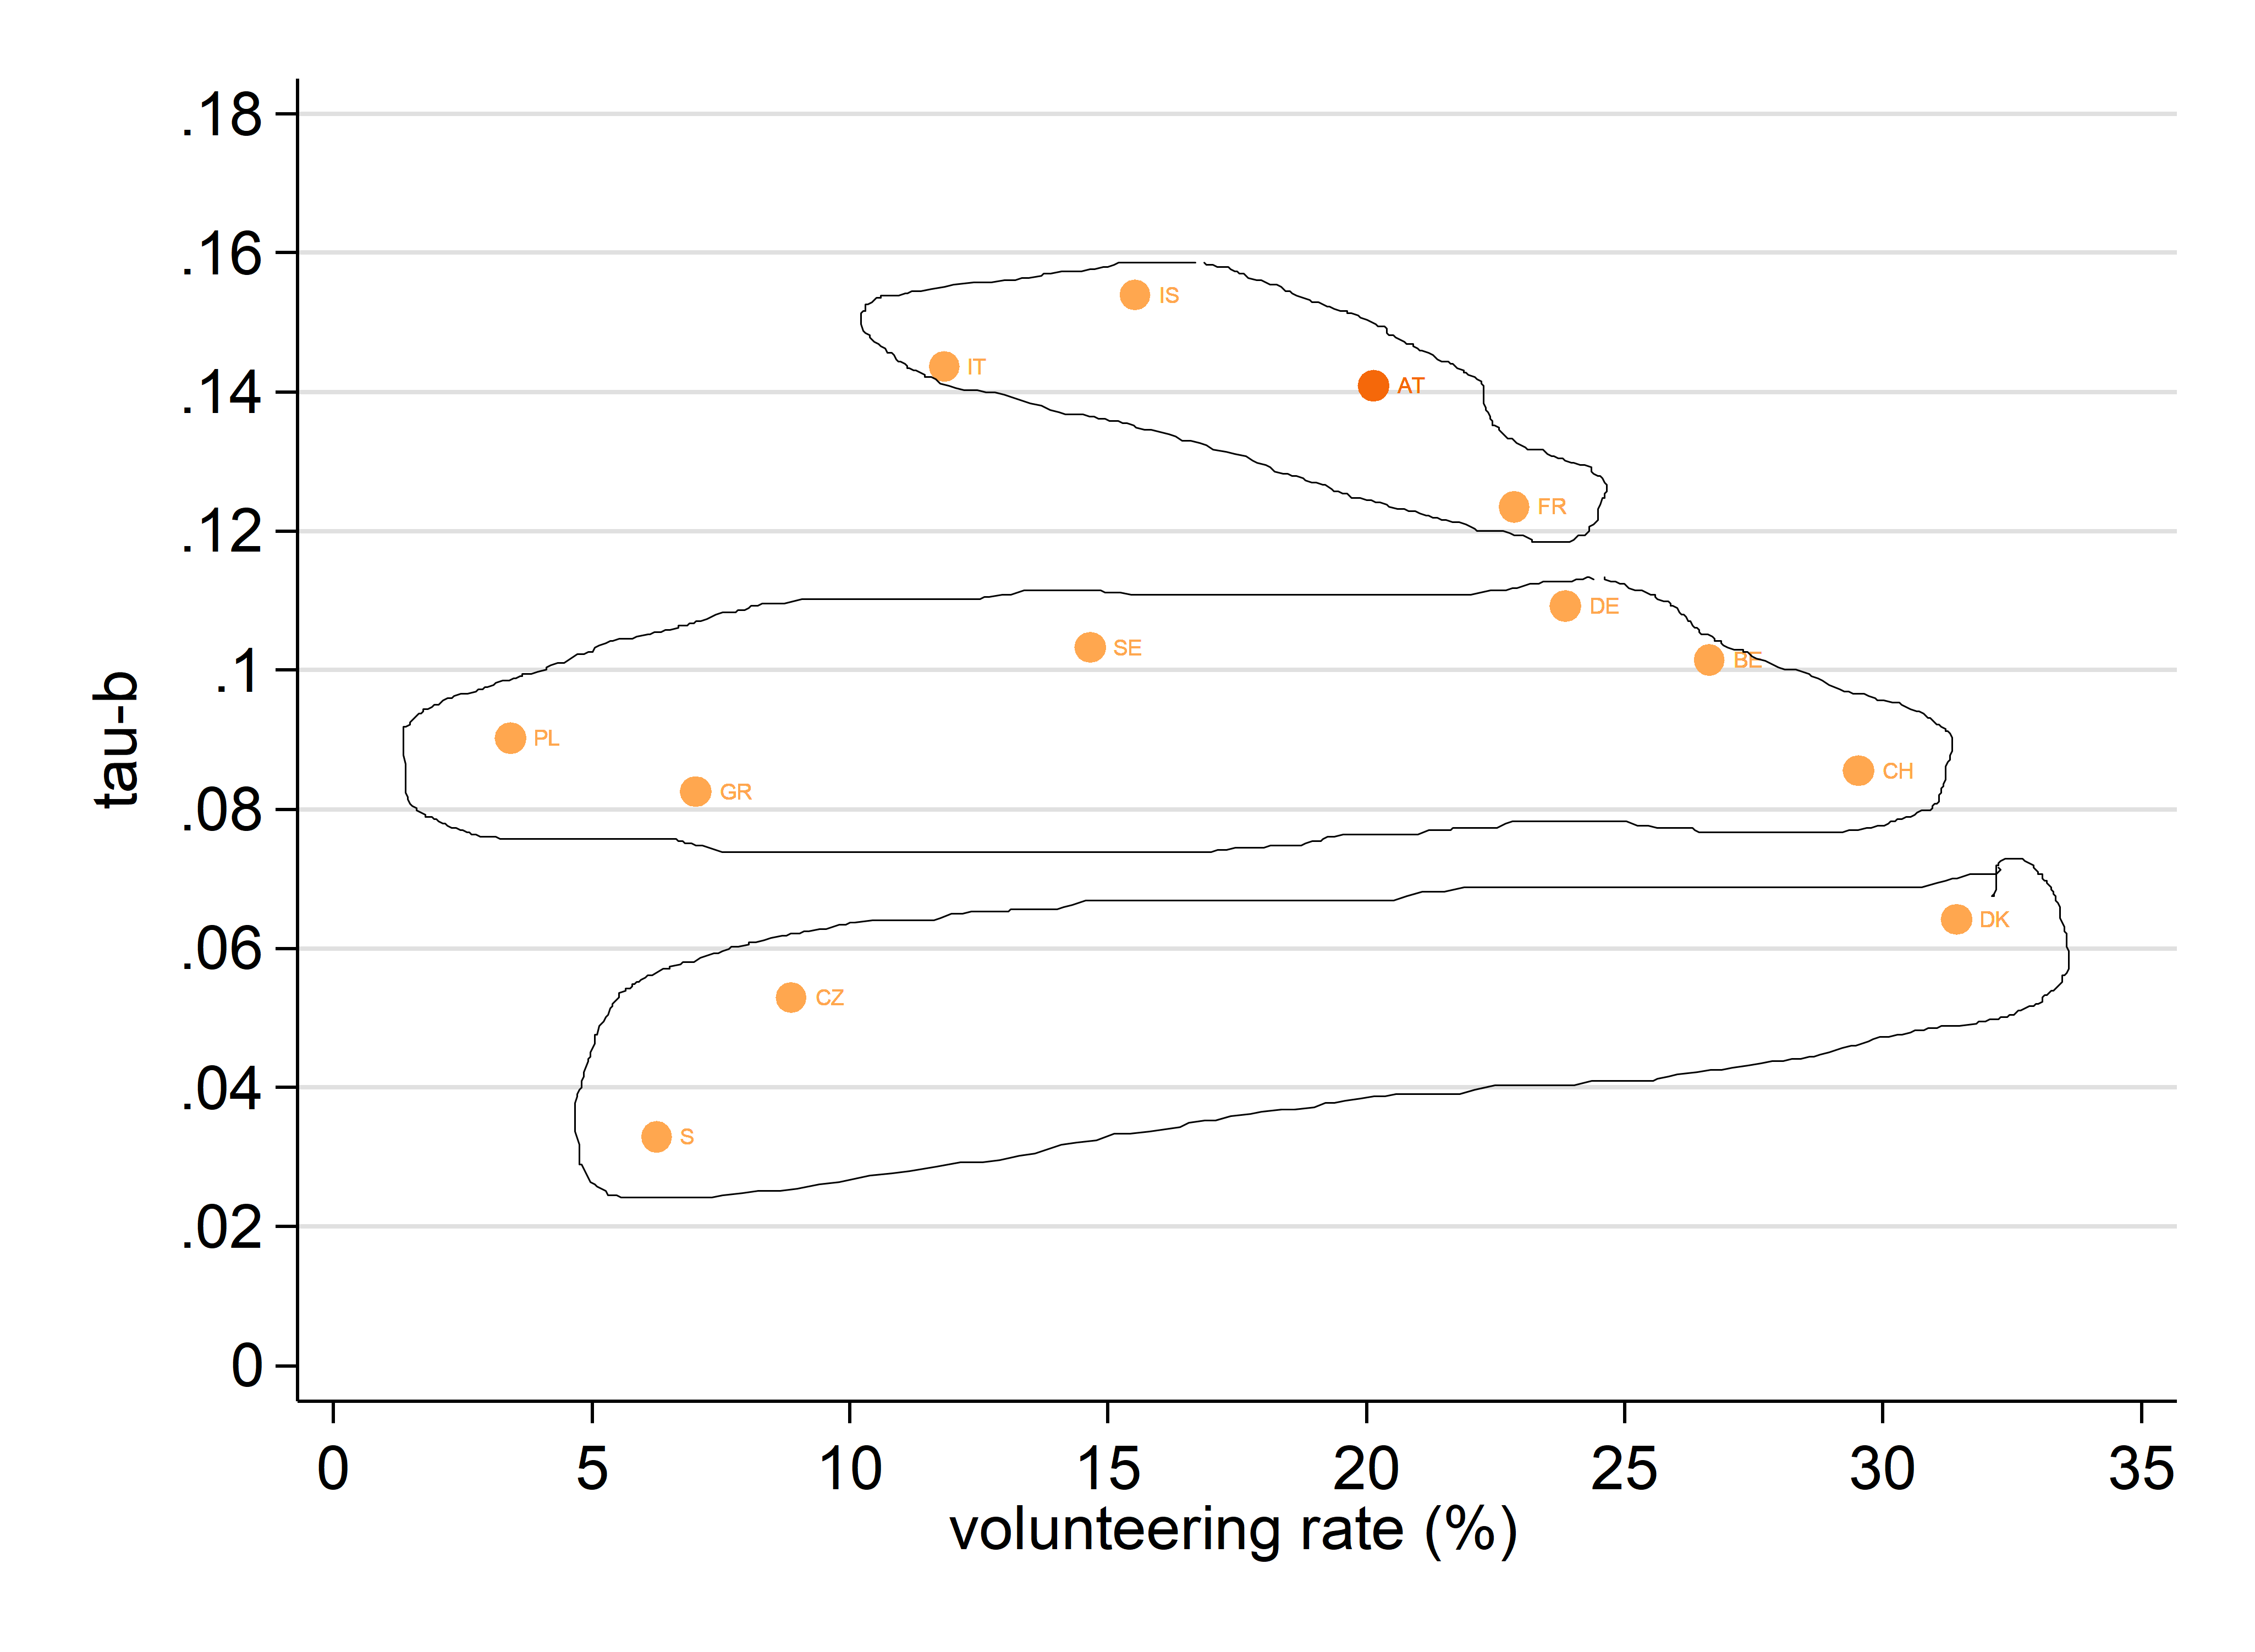
\includegraphics[height=3in]{Kendall_casp_petla.png}
 \centering
 \label{fig:tauLS}
\caption{tau Life satisfaction}
\end{figure}

A simple graphical presentation ( \ref{fig:tauLS} ) suggests nonlinear (quadratic) relatio between volunteering rate and impact of volunteering on life satisfaction. Association between volunteering and its relation with quality of life seems to be non-linear with an inverted U shape and the maximum association for the volunteering rate around 15\%. There is a decreasing association between volunteering and quality of life when the volunteering rates are higher. Since rate of volunteering is ralated to economic development we may expect a simalar relation between economic development and way how volunteering influences life satisfaction. The simplest way to check that relation is to regress GDP per capita (in PPP units) on life satisfaction measure (CASP). 

Two different  associations between volunteering and subjective health and quality of life are observed.  There is clear division into two groups in case of a subjective health. Denmark makes some puzzle for an analysis since the picture \textit{would have looked} better if the rate for Denmark either had been my a few percentages higher or the volunteering rate had been about 20\%. One can also consider existence country specific factors other than volunteering rate for countries such as Israel and Poland or Greece and Sweden. Below regression results of impact of interaction between volunteering and country volunteering rate on CASP are presented. 


%%% TABLE
\begin{spacing}{.9}
\begin{table}[H]
\centering 
\caption{CASP vs. volunteering and countrys' volunteering rates}  
\begin{scriptsize} 
	\begin{tabular}{p{1.8in}p{.5in}p{.5in}p{.5in}p{.5in}p{.5in}p{.5in}p{.5in}p{.5in}p{.5in}p{.4in}p{.5in}p{.4in}}\hline
	 {
\def\sym#1{\ifmmode^{#1}\else\(^{#1}\)\fi}
\begin{tabular}{l*{1}{c}}
\hline\hline
                    &\multicolumn{1}{c}{(1)}\\
                    &\multicolumn{1}{c}{casp}\\
\hline
vol                 &        0.50   \\
v1volrate           &        4.95   \\
v1volrate2          &       -8.39   \\
ageint              &       -0.01   \\
Male or female      &       -0.00   \\
yedu\_av             &        0.11*  \\
o.sphus==-1         &        0.00   \\
sphus==1            &        6.21***\\
sphus==2            &        4.87***\\
sphus==3            &        3.84***\\
sphus==4            &        2.13***\\
o.sphus==5          &        0.00   \\
averageGDP          &        0.10+  \\
avGDP2              &       -0.00   \\
constant            &       27.12***\\
\hline
N                   &       46485   \\
\hline\hline
\end{tabular}
}

      \hline\multicolumn{5}{l}{+p$<$0.10 *p$<$0.05 **p$<$0.01 ***p$<$0.001, robust std err} 		 	\end{tabular}
      \label{regB} 
\end{scriptsize}\end{table}
\end{spacing}
%%%% END: TABLE

\begin{figure}[H]
 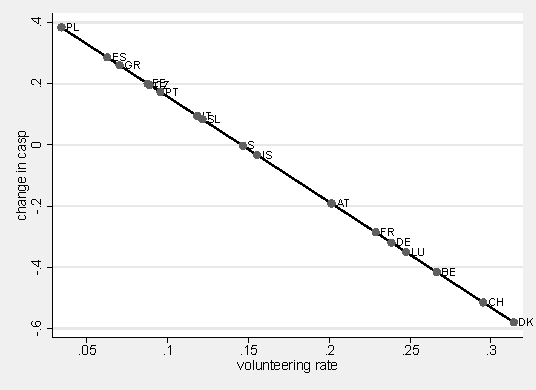
\includegraphics[height=3in]{regHm1.pdf}
 \centering\label{fig:m1}
\caption{}
\end{figure}
 
On average those engagaged in volunteering are more satisified with life than those who do not particiapate in such activity. The difference is the highest among countries with mid range volunteering rates (IT, SE, IS). In countries with little volunteering or high level of it the impact from volunteering on caspe is lower.   

\subsection{Result 3: Regression or multilevel approach to relation between Kendal(CASP, rate) and rate }

Another method to investigate relation between volunteering, economic development and life satisfaction is too estimate multilevel regression in which we allow for two random effects. This is varying-intercept and varying coefficient model. The varying-intercept is due to general differences among countries effect and  varying coefficient assumes that impact of volunteering on casp depends on gdp per capita. The model specification is: 

%
%\begin{itemize}
%\item Model 1 : Varying-intrcept model \footnote{Variance parameters are returned by xtmixed as logarithms of standard deviations in e(b). To tabulate the parameters as standard deviations, back-transform them using the transform() option} \\
%
% \begin{eqnarray}
%	casp_{ij}\sim N(c_{j}+\alpha * vol_{i}+\beta_{1}*age_{i}+\beta_{2}*gender_{i}+\sum \delta_k*h_{ik},\sigma^{2}_{y}) \\
%	c_{j} \sim N(\gamma_{0},sigma^{2}_{c})
% \end{eqnarray}
%
%%%% TABLE
%\begin{spacing}{.9}
%\begin{table}[H]
%\centering 
%\caption{CASP vs. volunteering and gdp per capita}  
%\begin{scriptsize} 
%	 \begin{tabular}{l*{1}{cc}} \hline\hline
             &\multicolumn{2}{c}{(1)}  \\
             &\multicolumn{2}{c}{casp} \\
\hline
vol          &       0.764&    (0.0636)\\
ageint       &     -0.0114&   (0.00277)\\
gender       &      -0.119&    (0.0487)\\
o.\_Isphus\_2  &           0&         (.)\\
\_Isphus\_3    &       6.054&     (0.189)\\
\_Isphus\_4    &       4.991&     (0.179)\\
\_Isphus\_5    &       3.643&     (0.176)\\
\_Isphus\_6    &       1.895&     (0.180)\\
o.\_Isphus\_7  &           0&         (.)\\
\_cons       &       36.14&     (0.691)\\
sd(Country)  &       2.295&     (0.451)\\
sd(Residual) &       4.407&    (0.0171)\\
\hline
\(N\)        &       33179&            \\
\hline\hline
\multicolumn{3}{l}{\footnotesize Standard errors in parentheses}\\
\end{tabular}

%      \label{regB} 
%\end{scriptsize}
%\end{table}
%\end{spacing}
%%%%% END: TABLE
%
%\item[a.] positive effect of volunteering on casp  
%\item[b.]  $\sigma_{y}=4.14$, $\sigma_{c}=2.34$
%\item[c.] LR test vs. linear model: chibar2(01) = 8244.90 (0.0000)
%\end{itemize}
%
%
% Model 2 : Varying-intercept and varying coefficient model
%
% \begin{eqnarray}
%	casp_{ij}\sim N(c_{j}+\alpha_{j} * vol_{i}+\beta_{1}*age+\beta_{2}*gender+\sum \delta_k*h_{ik},\sigma^{2}_{y}) \\
%	c_{j} \sim N(\gamma_{c},sigma^{2}_{c}) \\
%	\alpha_{j} \sim N(\gamma_{v},sigma^{2}_{v})
% \end{eqnarray}
%
%%%% TABLE
%\begin{spacing}{.9}
%\begin{table}[H]
%\centering 
%\caption{CASP vs. volunteering and gdp per capita}  
%\begin{scriptsize} 
%	 \begin{tabular}{l*{1}{cc}} \hline\hline
             &\multicolumn{2}{c}{(1)}  \\
             &\multicolumn{2}{c}{casp} \\
\hline
vol          &       0.947&     (0.180)\\
ageint       &     -0.0113&   (0.00276)\\
gender       &      -0.129&    (0.0487)\\
o.\_Isphus\_2  &           0&         (.)\\
\_Isphus\_3    &       6.065&     (0.189)\\
\_Isphus\_4    &       5.003&     (0.179)\\
\_Isphus\_5    &       3.649&     (0.176)\\
\_Isphus\_6    &       1.901&     (0.180)\\
o.\_Isphus\_7  &           0&         (.)\\
\_cons       &       36.15&     (0.711)\\
sd(vol)      &       0.599&     (0.141)\\
sd(cry)      &       2.372&     (0.466)\\
cov(vol,cry) &      -1.293&     (0.391)\\
sd(Residual) &       4.403&    (0.0171)\\
\hline
\(N\)        &       33179&            \\
\hline\hline
\multicolumn{3}{l}{\footnotesize Standard errors in parentheses}\\
\end{tabular}

%      \label{regB} 
%\end{scriptsize}
%\end{table}
%\end{spacing}
%%%%% END: TABLE
%
%\begin{itemize}
%
%\item[a.] positive effect of volunteering on casp  
%\item[b.]  $\sigma_{y}=4.40$, $\sigma_{c}=2.37$, $\sigma_{vol}=0.60$, $cov(vol, cry)=-1.30 $
%\item[c.] LR test vs. linear model: chibar2(01) = 8244.90 (0.0000)
%\item[d.] not much sense in covariance since cry is unordered ordinal variable

 \begin{eqnarray}
	casp_{ij}\sim N(\beta_{0}+c_{j}+ \alpha_{0}* vol_{i} + \alpha_{j} * vol_{i}+\beta_{1}*age_{i}+\beta_{2}*gender_{i}+\sum \delta_k*h_{ik},\sigma^{2}_{y}) \\
	c_{j} \sim N(\gamma_{c},\sigma^{2}_{c}) \\
	\alpha_{j} \sim N(\gamma_{v}*volrate_{j},\sigma^{2}_{v})
 \end{eqnarray}

There are levels of data in the model. The level one is the individual level and the level two are countries. We assume a random intercept for each country (level 2 cluster) what means a different average casp for individuals living within a country after controlling for gender, age and other independent variables. We allow for a variation among those averages. Country effect in life satisfaction regression has been intensively studied in literature (blef ... literature is needed). Varying slope assumption means that impact of being active in volunteering can have different impact on casp depending on then country volunteering rate. \\

In the model volunteering influences casp through fixed effect of  $\alpha_{0}$ and through country specific parameter $\alpha_{j}$ that depends on the country volunteering rate. 

%%% TABLE
\begin{spacing}{.9}
\begin{table}[H]
\centering 
\caption{CASP vs. volunteering and gdp per capita}  
\begin{scriptsize} 
	 {
\def\sym#1{\ifmmode^{#1}\else\(^{#1}\)\fi}
\begin{tabular}{l*{1}{c}}
\hline\hline
            &\multicolumn{1}{c}{(1)}\\
            &\multicolumn{1}{c}{casp}\\
\hline
vol         &        0.91***\\
age         &       -0.01***\\
female      &       -0.10*  \\
edu         &        0.06***\\
o.\_Isphus\_2 &        0.00   \\
\_Isphus\_3   &        6.79***\\
\_Isphus\_4   &        5.72***\\
\_Isphus\_5   &        4.35***\\
\_Isphus\_6   &        2.38***\\
o.\_Isphus\_7 &        0.00   \\
income      &        0.00***\\
averageGDP  &        0.26***\\
avGDP2      &       -0.00** \\
\_IcountrySH\_2&       -1.78***\\
\_IcountrySH\_3&       -0.14   \\
\_IcountrySH\_4&       -1.56***\\
\_IcountrySH\_5&       -0.85***\\
\_IcountrySH\_6&       -6.87***\\
\_IcountrySH\_7&       -4.42***\\
\_IcountrySH\_8&       -3.87***\\
\_IcountrySH\_10&       -2.48***\\
\_IcountrySH\_11&       -1.21***\\
\_IcountrySH\_12&        1.75+  \\
\_IcountrySH\_13&       -3.06***\\
\_IcountrySH\_14&        1.44** \\
\_IcountrySH\_16&       22.54** \\
\_IcountrySH\_18&       -3.01***\\
o.\_IcountrySH\_19&        0.00   \\
o.\_IcountrySH\_20&        0.00   \\
o.\_IcountrySH\_47&        0.00   \\
constant    &       22.91***\\
sd(vol)     &        0.22***\\
sd(Residual)&        4.52***\\
\hline
N           &       45764   \\
\hline\hline
\end{tabular}
}

      \label{regB} 
\end{scriptsize}
\end{table}
\end{spacing}
%%%% END: TABLE

For each country we may calculate a marginal effect of volunteering on casp as $\hat{\alpha_{0}}+\hat{u_{vj}} $

\begin{figure}[H]
 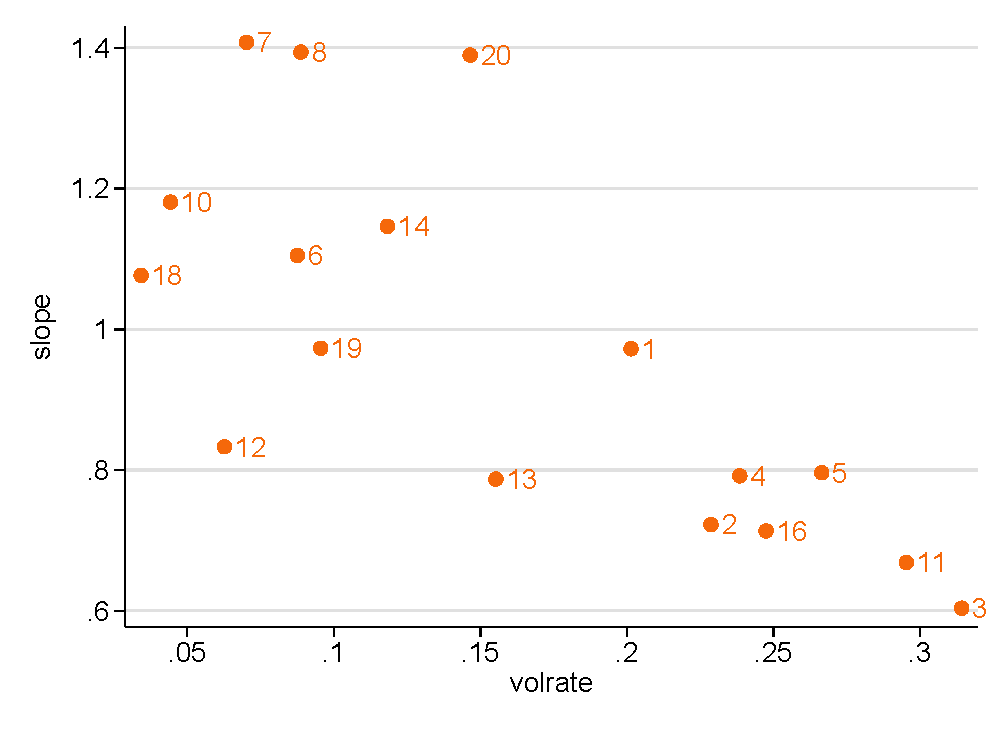
\includegraphics[height=3in]{regHm3_slope.pdf}\centering\label{fig:m3}
\caption{}
\end{figure}

Results are promising. Low marginal efferct for Sweden and Czech Republic. The largest for Italy and Isreal. Large for Sweden. Small values for large volunteering rates (AT, ...,DK). 

\section{Discussion}

The positive consequences of being engaged in volunteering by elderly are well known and commonly accepted. Volunteering is important and it needs to be study in details.  According to OECD estimates the value of unpaid volunteering ranges from X\% of GDP to as much as Y\% (OECD, yyyy).  Demographic changes combined with progress in health care add to increasing time while people are in relatively good health while being on retirement. This creates additional  stock of unused labor among elderly that may be effectively used with benefit for volunteer and other members of a society.  It makes   volunteering of elderly to be potentially important policy tool that may help to keep people in better health when they get older. \\


Casual realtion between volunteering  and health or wellbeing is not obvious. Volunteering may improve the employability of volunteers and it provides engagement in a socially meaningful role  what could positively impact on health and well-being. Volunteering might builts up social networks and gives meaning and purpose in life. (przepisana, zmodyfikowane) //

The question that must be asked is whether popularization of volunteering should be put into social policy agenda. Taking into consideration our results we expect different answers in different countries. It is possible that in some rich and highly developed countries volunteering is so popular and treated as so usuall activity that it adds only marginally to individuals' wellbeing. 

\section{Literature}


\section{Statistical Appendix}

1. Kendall tau b \\
2. Multilevel Linear Regresion Model

\end{spacing}
\end{document}
